Halo dan selamat datang di pembelajaran neural jaringan convolutional canggih dalam Python bagian 9
ini adalah salah satu kursus paling menarik yang pernah saya lakukan dan itu benar-benar menunjukkan seberapa cepat dan seberapa dalam belajar
telah datang.

Selama bertahun-tahun ketika saya pertama kali memulai seri pembelajaran mendalam saya, saya tidak pernah menganggap bahwa saya akan membuat dua seri
kursus tentang jaring convolutional tetapi saya pikir apa yang akan Anda temukan adalah bahwa kursus ini sangat berbeda
dari yang sebelumnya.

Anda akan terkesan dengan betapa banyak materi yang harus kita bahas dan sebesar ini, tentu saja saya masih
punya lebih banyak ide yang ingin saya tambahkan sebagai pembaruan di masa depan.
Jadi izinkan saya memberi Anda ringkasan singkat tentang apa kursus ini.
Pertama kita akan menjembatani kesenjangan antara arsitektur CNN dasar yang sudah Anda kenal dan sukai
arsitektur novel modern seperti Viji Reznick dan Inception yang mungkin sudah Anda duga namanya
setelah film.

Kita akan menerapkan ini pada gambar sel darah dan membuat sistem yang memiliki ahli medis yang lebih baik
daripada Anda atau saya.
Itu ide yang cukup rapi jika Anda berpikir bahwa dokter masa depan bukanlah manusia tetapi robot.
Kedua, salah satu tema utama dari kursus ini adalah kita beralih dari CNN ke sistem
melibatkan CNN.

Jadi apa yang saya maksud dengan itu.
CNN melakukan satu klasifikasi gambar hal dasar dalam kursus ini, Anda akan melihat bagaimana kita dapat mengubah CNN
ke dalam sistem deteksi objek yang tidak hanya mengklasifikasikan gambar tetapi dapat menemukan setiap objek dalam suatu gambar
dan prediksi labelnya.

Anda dapat membayangkan bahwa tugas seperti itu merupakan prasyarat dasar untuk kendaraan yang bisa menyetir sendiri.
Kita akan melihat algoritma canggih yang disebut SSD tugas penglihatan komputer yang sangat populer
yang memanfaatkan CNN'S disebut transfer gaya neuros.

Di sinilah Anda mengambil satu gambar yang disebut gambar konten dan gambar lain disebut gambar gaya
dan Anda menggabungkan ini untuk membuat gambar yang sama sekali baru seolah-olah Anda menyewa seorang pelukis untuk melukis konten
dari gambar pertama dengan gaya yang lain tidak seperti pelukis manusia.
Ini bisa dilakukan dalam hitungan detik.
Saya harap Anda senang mempelajari aplikasi canggih CNN ini.
Sampai jumpa di kelas.


\section{Jaringan saraf convolutional canggih}
Tujuan Pembelajaran
\begin{enumerate}

\item  kita telah melihat bahwa 3-5 layer netscan membutuhkan waktu yang sangat lama untuk dilatih
(tapi sekarang kita akan melihat 50 layer nets)
\item penelitian hari ini (dalam pembelajaran mesin) berkomitmen untuk keterbukaan, dan dengan membagikan penelitian mereka, mudah bagi Anda untuk melakukan hal-hal canggih di rumah
(Tidak ada bidang lain yang bisa mencapai ini: biologi, kedokteran, fisika, ...dan lain sebagainya)
\item kita dapat menggunakan bobot pra-terlatih menggunakan transfer belajar secara signifikan mengurangi waktu pelatihan karena kita sekarang hanya perlu melakukan fine-tuning
\end{enumerate}

\section{cara untuk melakukan kursus ini dengan baik}
Saya telah menemukan solusi ini setelah mengamati siswa/i selama bertahun-tahun,
pada umumnya, mereka yang mengikuti solusi ini telah mendapatkan kesuksesan, mereka yang memiliki masalah disebabkan karena tidak mengikuti solusi ini.

Hal-hal atau solusi yang diperlukan antara lain :
\begin{enumerate}
\item memanfaatkan dengan adanya Question and Answer  
\item memerlukan waktu respon yang cepat
\item mempunyai motifasi yang tinggi
\item menggunakan sotfware yang kita mengerti dan kita pahami 
\end {enumerate}

\section{cara untuk mendapatkan kode dan data}
Langkahnya sebagai berikut
\begin{figure}[!htp]
	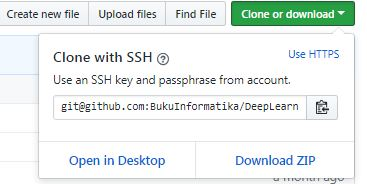
\includegraphics[width=0.75\textwidth]{figures/ssh.JPG}
	\caption{contoh pengambilan kode ssh}
	\label{labelgambar}
\end{figure}

\begin{enumerate}
\item mengambil kode ssh yang ada pada github dan pastikan yang dicopy adalah ssh bukan https
\item jangan lupa melakukan fork terlebih dahulu
\item kemudian disarankan untuk tidak memalsukan repo karena dapat mempersulit 
\end{enumerate}

Dalam hal data, data akan kita temui pada saat kita dalam kuliah dan kursus, beberapa siswa telah meminta saya untuk memberikan 
tentang tutorial latihan coding dalam kursus ini jadi tidak ada alasan lagi untuk tidak dapat mengoding